%!TEX root = paper.tex

\section{Introduction} % (fold)
\label{sec:introduction}

Automatic loop invariant inference is a fundamental program analysis problem, 
which is useful in software verification, test-case generation, 
compiler optimization, program understanding, etc. 
Previous research on invariant inference mainly uses 
abstraction interpretation~\cite{cite}, 
counterexample guided abstraction refinement~\cite{cite}, 
interpolation-based approaches~\cite{cite}, 
and constraint-based inference~\cite{cite}. 
In this work, we propose a new invariant inference framework 
that actively learns the loop invariant from the runtime data using machine learning. 
By combining selective sampling~\cite{cite}, 
support vector machine learning~\cite{cite}, 
concolic testing~\cite{sen2007concolic} 
and constraint solving~\cite{cite}, 
we refine the inferred loop invariant after each iteration 
until it converges and proves the property preserved by the loop program. 

Generally, a loop program $P$ can be written in the following form, 
where $\mathit{Pre}$, $\mathit{Cond}$ and $\mathit{Post}$ are boolean conditions, 
and $\mathit{Body}$ is the loop body. 
%\[
%    P = \{ \mathit{Pre} \} \mathit{while}(\mathit{Cond}) \{ \mathit{Body} \} \{ \mathit{Post} \}
%\]
\begin{align*}
&\mathit{assume}(\mathit{Pre}) & & /\star\text{\emph{Assumption}}\star/ \\
&\mathit{while} (\mathit{Cond}) \{ && \\
&\quad \mathit{Body} & & /\star\text{\emph{Loop Body}}\star/ \\
&\} && \\
&\mathit{assert}(\mathit{Post}) & & /\star\text{\emph{Assertion}}\star/ 
\end{align*}
In practice, the pre-condition $\mathit{Pre}$ is often described by 
the specification documents and checking conditions of the program inputs, 
and the post-condition $\mathit{Post}$ is usually specified 
by assertions and exceptions leading to an error state in the program. 
Let $s = \{ x_1 \mapsto v_1, \ldots, x_n \mapsto v_n \}$ represent 
the evaluation function of the program variables $x_1, \ldots, x_n$
and $\mathit{Body}(s)$ stand for their new evaluation after the execution of $\mathit{Body}$, 
the above program means that (1) $\mathit{Pre}$ is the assumption to the initial value of $s$; 
(2) if the $\mathit{Cond}$ is satisfied by $s$ at an iteration, 
$\mathit{Body}$ will be executed and $s$ will be updated to $\mathit{body}(s)$; 
(3) if the $\mathit{Cond}$ is unsatisfied by $s$ at an iteration, 
the while-loop ends and $s$ should satisfy $\mathit{Post}$. 
To prove the correctness of the above program specification, 
we need to find a loop invariant $\mathit{Inv}$ that meets the following three conditions. 
\begin{align}
    &s \models \mathit{Pre} 
        &&\Longrightarrow & s &\models \mathit{Inv} \label{inv:pre} \\
    &s \models \mathit{Inv} \wedge \mathit{Cond} 
        &&\Longrightarrow & \mathit{Body}(s) &\models \mathit{Inv} \label{inv:loop} \\
    &s \models \mathit{Inv} \wedge \neg\mathit{Cond} 
        &&\Longrightarrow & s &\models \mathit{Post} \label{inv:post}
\end{align}
The goal of this work is to develop an  automatic learning method of 
the invariant $\mathit{Inv}$ from the loop program and thus prove its correctness. 

\begin{figure}[t]
\begin{subfigure}{0.2\textwidth}
    \centering
    \vspace{0.5cm}
{\scriptsize\begin{verbatim}
void P(int x, int y) {
    assume(x < y);
    while (x < y) {
        if (x < 0) x = x + 7;
        else x = x + 10;
        
        if (y < 0) y = y - 10;
        else y = y + 3; 
    }
    assert(x >= y
        && x <= y + 16);
}
\end{verbatim}}
    \vspace{0.5cm}
    \caption{Loop Program}
    \label{fig:running:example:program}
\end{subfigure}%
\begin{subfigure}{.3\textwidth}
      \centering
      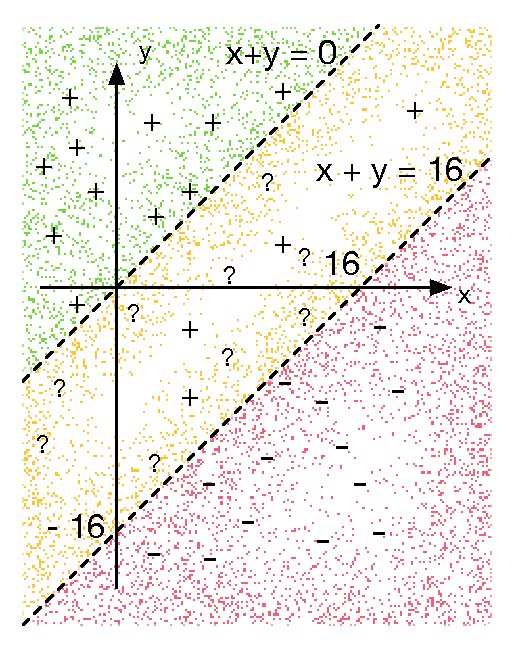
\includegraphics[scale=0.42]{figures/running-sampling.pdf}
      \caption{Sampling}
      \label{fig:running:example:sampling}
\end{subfigure}
\caption{A Running Example}
\label{fig:running:example}
\end{figure}

\begin{figure}[t]
    \centering
    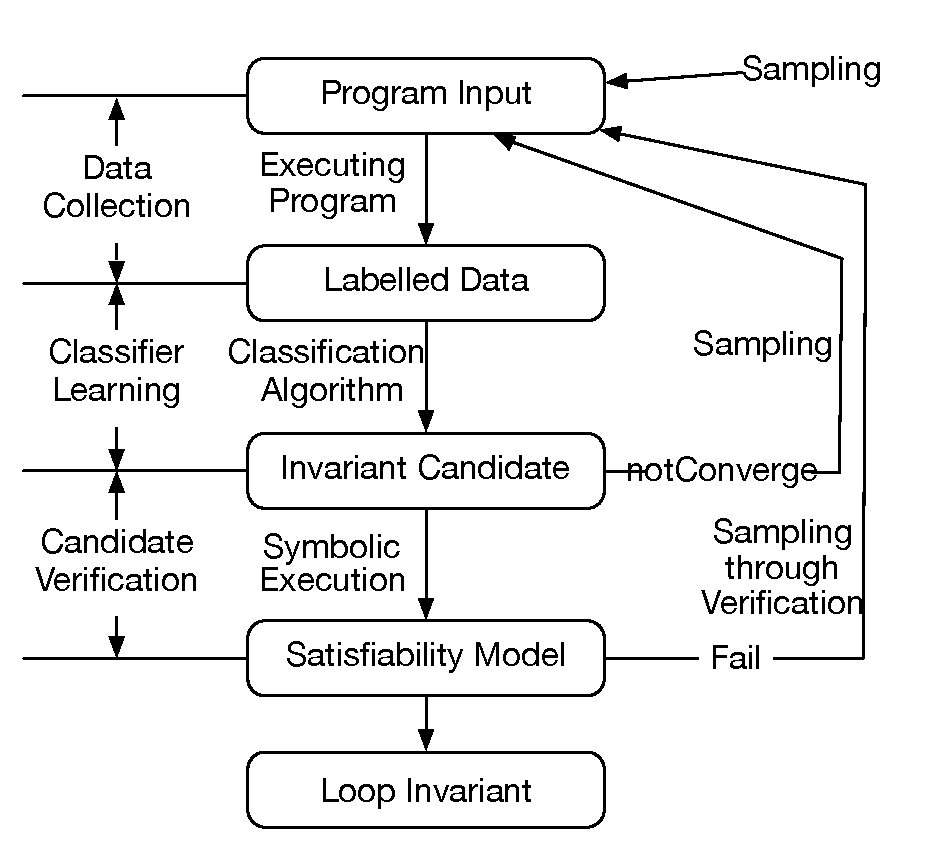
\includegraphics[scale=0.45]{figures/overview.pdf}
    \caption{Loop Invariant Inference Framework Overview}
    \label{fig:overview}
\end{figure}

\medskip\noindent
\textbf{A Running Example}
is shown in Figure~\ref{fig:running:example:program}. 
The loop program $P$ takes two integer variables $x$ and $y$ as inputs. 
The assumption $\mathit{Pre}$ requires that $x < y$, 
which is the same as the loop condition $\mathit{Cond}$. 
When $\mathit{Cond}$ is met in each loop iteration, 
$x$ is increased by $7$ if $x$ is negative, otherwise $x$ is increased by $10$; 
$y$ is decreased by $10$ if $y$ is negative, otherwise $y$ is increased by $3$. 
Finally, the assertion of $P$ specifies that 
$y \le x \le y + 16$ should be true when the loop ends. 
The correctness of the program specification in Figure~\ref{fig:running:example} 
can be proven by checking the three conditions 
(\ref{inv:pre}), (\ref{inv:loop}) and (\ref{inv:post}) above 
with a loop invariant $\mathit{Inv} = x \le y + 16$ (or $2 \times x \le 2 \times y + 33$, etc). 
We use this running example in the following 
to illustrate different stages of our invariant reference method. 

\medskip\noindent
\textbf{Overview.}
Our framework treats the invariant reference as an active learning and refinement process 
based on iterations of data collection, active learning and invariant verification 
as shown in the Figure~\ref{fig:overview}. 
Let $P$ be the loop program. 
\begin{itemize}
    \item 
    % (1)
    In the \textbf{Data Collection} stage (see Section~\ref{sec:sampling}), 
    we first obtain program inputs $S_{\mathit{in}}$ from three kinds of sampling sources: 
    random sampling, selective sampling and counter-example sampling. 
    Then, given an input $s_0$ in $S_{\mathit{in}}$, we execute $P$ with $s_0$ 
    and record the evaluations of variables for all of the loop iterations
    as a trace $\langle s_0, s_1, \ldots, s_n \rangle$.  
    All of the evaluations in the above trace (referred by its initial evaluation $s_0$) 
    are labelled based on a pair of boolean values 
    $(s_0 \models \mathit{Pre}, s_n \models \mathit{Post})$\footnote{
        $(\mathit{true}, \mathit{true}) \rightarrow +$, 
        $(\mathit{false}, \mathit{false}) \rightarrow -$ 
        and $(\mathit{false}, \mathit{true}) \rightarrow ?$}. 
    The regions of inputs with different labels for our running example can be intuitively shown 
    in Figure~\ref{fig:running:example:sampling} with different colors. 
    Given the above evaluation trace with
    $s_0 \models \mathit{Pre}$ and $s_n \not\models \mathit{Post}$, 
    our framework returns it as a proof of the program specification error. 
    \item 
    % (2) 
    Based on the labelled evaluations from the \emph{data collection} stage, 
    we \emph{actively} learn a classifier to capture the positive ones from the negative ones 
    using machine learning algorithms, e.g., SVM derivatives, 
    in the \textbf{Active Learning} stage (see Section~\ref{sec:learning}). 
    When the recently learnt classifier converges to the previously learnt ones, 
    we treat it as an invariant candidate and move to the next stage. 
    Otherwise, we apply selective sampling on the recently learnt classifier 
    to add more samples to $S_{\mathit{in}}$. 
    When a sample cannot be classified using a certain classification model, 
    we try other alternative models in a sequential order. 
    \LL{We prove the termination of the \emph{active learning} stage if such an invariant exists.}
    \item 
    % (3) 
    When an invariant candidate is found, we check its correctness 
    in the \textbf{Invariant Verification} stage (see Section~\ref{sec:verification}). 
    First, we check condition (\ref{inv:pre}) and condition (\ref{inv:post}) with the candidate. 
    Then, we verify the condition (\ref{inv:loop}) 
    based on all of the program execution traces of $\mathit{Body}$ using symbolic execution~\cite{}. 
    The above conditions are checked by SMT~\cite{barrett2009satisfiability} solvers in this work. 
    If all of the above conditions are satisfied, 
    we claim the correctness of $P$ with its loop invariant. 
    Otherwise, we add the counter-example from SMT Solving to $S_{\mathit{in}}$ 
    and restart from the \emph{data collection} stage. 
\end{itemize}


%The overall algorithm is shown in Algorithm~\ref{alg:overall}.
%\section {Overall Algorithm}
%\label{sec:overall}
% \LL{Do not put the algorithm here. It contains lots of notations undefined.}
% The overall algorithm is presented in Figure~\ref{alg:overall}.
% \begin{algorithm}[!h]
% \SetAlgoVlined
% \Indm
% \KwIn{$Pre$, $Cond$, $Body$, $Post$}
% \KwOut{an invariant which completes the proof or a counter-example}
% \Indp
% let $S$ be \textsc{Null}\;
% \While{true} {
%     add Samples into $S$\;
%     test the program for each sample in $S$\;
%     \If {a state $s$ in $\mathcal{S}^x$ is identified} {
%         \Return $s$ as a counterexample;
%     }
%     let $\mathcal{S}^+$, $\mathcal{S}^-$ and $\mathcal{S}^\rightarrow$ be respective sets accordingly\;
%     let $\mathcal{C}$ = activeLearning($\mathcal{S}^+$, $\mathcal{S}^-$, $\mathcal{S}^\rightarrow$)\;
%     Extract path constraints $\textsc{Pc}$ based on (1)(2)(3)\;
%     \For {each $pc$ in $\textsc{Pc}$} {
%         \If { $pc$ is not satisfied} {
%             add the counter-example into $S$\;
%             continue\;
%         }
%     }
%     \Return $\mathcal{C}$ as the proof;
% }
% \caption{Algorithm $overall$}
% \label{alg:overall}
% \end{algorithm}
%
% \begin{theorem}
% Algorithm $overall$ always eventually terminates and it is correct. \hfill \qed
% \end{theorem}


\medskip\noindent
\textbf{Contributions.}
Our contributions are four-fold. 
\begin{itemize}
    \item 
    We are the first to propose an active learning and refinement framework 
    for automatic invariant inference based on machine learning. 
    Since the samples are chosen for clear purpose 
    to refine the invariant candidate in the \emph{data collection} stage, 
    the invariant converges efficiently. 
    Furthermore, because the counter-examples generated in the \emph{invariant verification} stage 
    give very accurate information to amend the invariant candidate, 
    they become a useful supplementary to overcome the weakness of machine learning 
    and fine-tune the invariant candidate. 
    \item 
    Our framework is highly adaptable to different invariant inference scenarios 
    because the classification methods have a wide range of choices. 
    In this work, we show that linear, polynomial as well as 
    their conjunctive classification methods work effectively in our framework. 
    More importantly, our framework can be easily and intuitively extended with other alternative methods. 
    \item 
    Our framework can be practically used to verify real programs with ease, 
    as the samples are generated at runtime 
    and our framework is language/platform independent based on other tools 
    (e.g., GSL (GNU Scientific Library)~\cite{gough2009gnu} for selective sampling, 
    LibSVM~\cite{chang2011libsvm} for SVM classification, 
    Z3~\cite{de2008z3} for invariant verification 
    and KLEE~\cite{cadar2008klee} for concolic testing~\cite{sen2007concolic}). 
    \item 
    We implement our framework as a tool called \textsc{Zilu} 
    and compare it with other available state-of-the-art invariant inference tools, 
    i.e., CPAChecker~\cite{beyer2011cpachecker}, Interproc. 
    Our experiment results show that 
    we are the only tool that can work with polynomial invariant inference. 
    Notice that the polynomial invariant inference works in our framework 
    naturally with very light additional programming. 
    % Based on the design of different approaches,
    % we also claim that our framework have better extensibility comparing with their method.
\end{itemize}

\medskip\noindent
\textbf{Structure of this paper.}

% section introduction (end)